\documentclass[a4paper,  11pt]{ctexart}
\usepackage{srcltx,graphicx}
\usepackage{amsmath, amssymb, amsthm}
\usepackage{color}
\usepackage{lscape}
\usepackage{multirow}
\usepackage{psfrag}
\usepackage{diagbox}
\usepackage[hang]{subfigure}
\usepackage{float}
\usepackage{cases}
\usepackage[colorlinks,linkcolor=black,anchorcolor=blue,citecolor=green]{hyperref}

\newtheorem{theorem}{Theorem}
\newtheorem{lemma}{Lemma}
\newtheorem{definition}{Definition}
\newtheorem{comment}{Comment}
\newtheorem{conjecture}{Conjecture}

\newcommand\bbR{\mathbb{R}}
\newcommand\bbN{\mathbb{N}}
\newcommand\bbC{\mathbb{C}}
\newcommand\bx{\boldsymbol{x}}
\newcommand\dd{\,\mathrm{d}}

\newcommand\diag{\mathrm{diag}}
\newcommand\tr{\mthrm{tr}}

\setlength{\oddsidemargin}{0cm}
\setlength{\evensidemargin}{0cm}
\setlength{\textwidth}{150mm}
\setlength{\textheight}{230mm}

\newcommand\note[2]{{{\bf #1}\color{red} [ {\it #2} ]}}
%\newcommand\note[2]{{ #1 }} % using this line in the formal version

\newcommand\pd[2]{\dfrac{\partial {#1}}{\partial {#2}}}
\newcommand\od[2]{\dfrac{\dd {#1}}{\dd {#2}}}
\newcommand{\bm}[1]{\mbox{\boldmath{$#1$}}}

\begin{document}
\title{图像处理中的数学方法—homework3}
\author{郑灵超}
\maketitle
% \tableofcontents
% \newpage

\section{理论分析}
  水平集方法描述曲线演化的方程:
  \begin{align}
    \pd{u}{t}(t,x) = F|\nabla u(t,x)|, \quad t\geq 0,x\in\Omega, \\
    u(0,x)=\bar{d}(x,c_0),\\
    \pd{u}{N}=0,\quad t\geq 0,x\in\partial\Omega.
  \end{align}
  其中
  \[\bar{d}(x,c_0)=
  \begin{cases}
    +d(x,c_0) ,\quad x \text{在}c_0\text{外部},\\
    -d(x,c_0) ,\quad x \text{在}c_0\text{内部}.
  \end{cases}
  \]
  将水平集方法应用到$Geodesic active contours$模型中,得到的方程为
  \[
  \pd{u}{t}=g(|\nabla I|)\left(\text{div}\left(\frac{\nabla u}{
  |\nabla u|}\right)+\alpha\right)|\nabla u|+\langle\nabla g,\nabla
  u\rangle.
  \]
  其中$g(s)=\frac{1}{1+s^2}$.

  上式的离散格式为
  \[
  \begin{aligned}
    u_{i,j}^{n+1}=u_{i,j}^n + \Delta t \Big[ & g_{i,j}K_{i,j}^n
    [(\delta_x u_{i,j}^n)^2+(\delta_y u_{i,j}^n)^2]^{\frac 12} \\
    &
    +\alpha[\max(g_{i,j},0)\nabla^++\min(g_{i,j},0)\nabla^-]u_{i,j}^n\\
    &\max(g_{x_{i,j}},0)\delta_x^- u_{i,j}^n+\min(g_{x_{i,j}},0)\delta_x^+
    u_{i,j}^n \\
    &\max(g_{y_{i,j}},0)\delta_y^- u_{i,j}^n+\min(g_{y_{i,j}},0)\delta_y^+
    u_{i,j}^n \Big]
  \end{aligned}
  \]
其中 
\[
\begin{aligned}
  \nabla^+ u_{i,j}^n = \Big[
  &\max(\delta_x^-u_{i,j}^n,0)^2 
  +\min(\delta_x^+u_{i,j}^n,0)^2 \\
  &+\max(\delta_y^-u_{i,j}^n,0)^2 
  +\min(\delta_y^+u_{i,j}^n,0)^2 
  \Big]^{\frac 12}.
\end{aligned}
\]

\section{数值结果}
我们取得默认参数为$\alpha=1,dt=0.3,step=200$,并每10步做一次重初始化。
对以下几种情况,我们的测试结果如下:
\subsection{简单图形}
\begin{figure}[H]
    \centering
    \subfigure[原图]{
    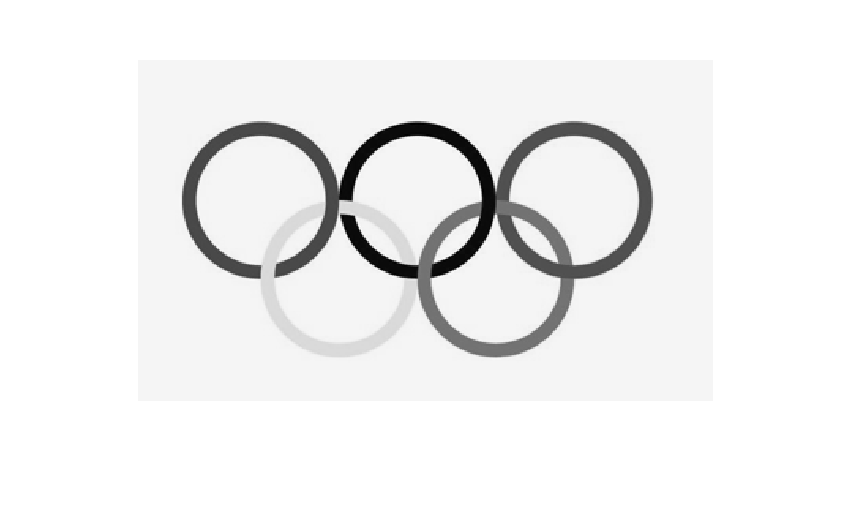
\includegraphics[width=0.45\textwidth]{../program/timg.eps}}
    \subfigure[迭代结果]{
    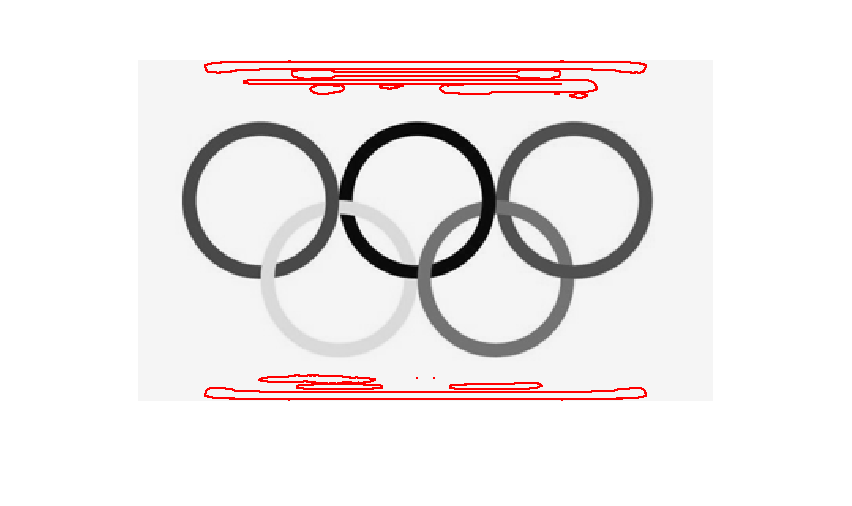
\includegraphics[width=0.45\textwidth]{../program/timg-1.eps}}
    \subfigure[得到的边界]{
    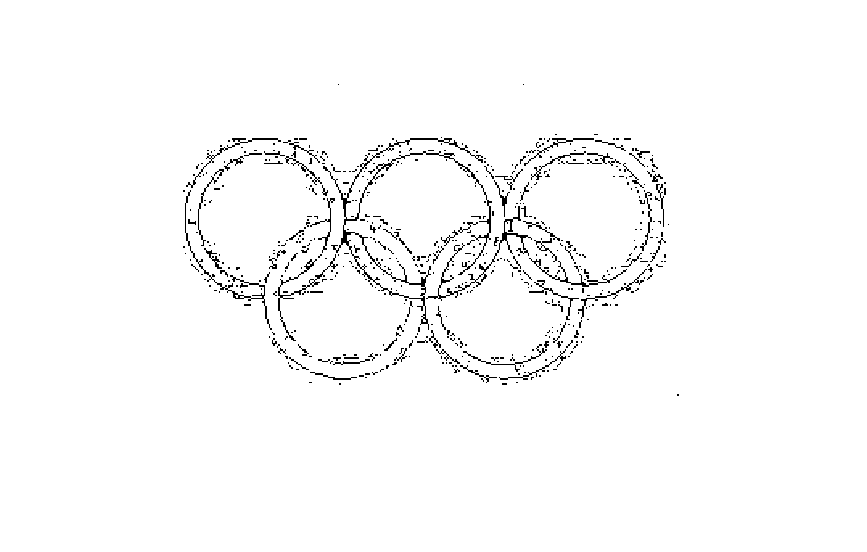
\includegraphics[width=0.45\textwidth]{../program/timg-2.eps}}
    \subfigure[梯度图]{
    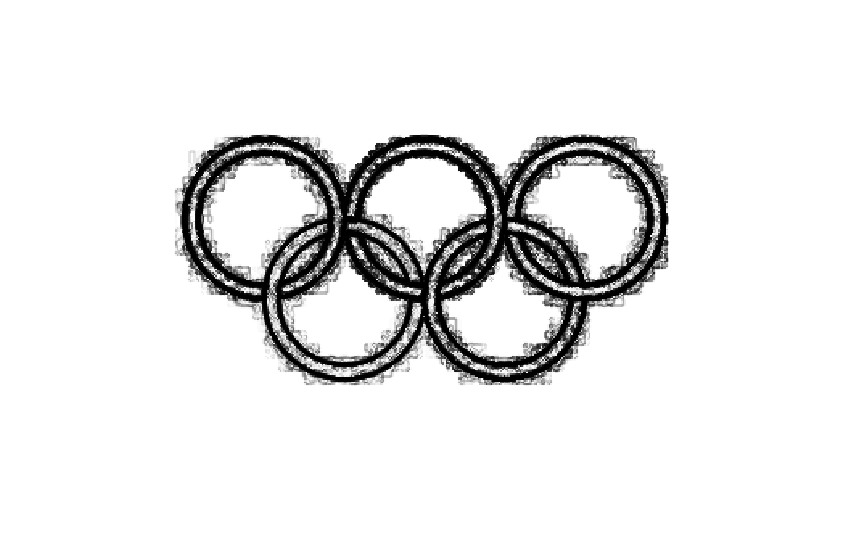
\includegraphics[width=0.45\textwidth]{../program/timg-3.eps}}
\end{figure}
可以发现对简单图形,利用水平集方法对其进行逼近的效果较好,利用梯度也可
以大致看出图像的轮廓。
\subsection{分离图形}
\begin{figure}[H]
    \centering
    \subfigure[原图]{
    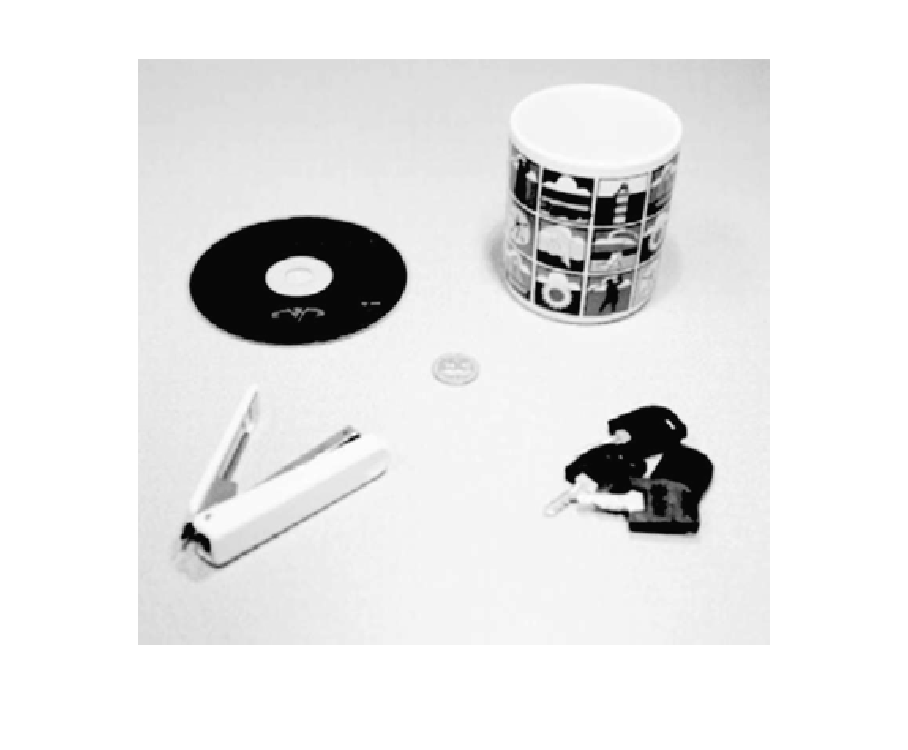
\includegraphics[width=0.45\textwidth]{../program/wenju.eps}}
    \subfigure[迭代结果]{
    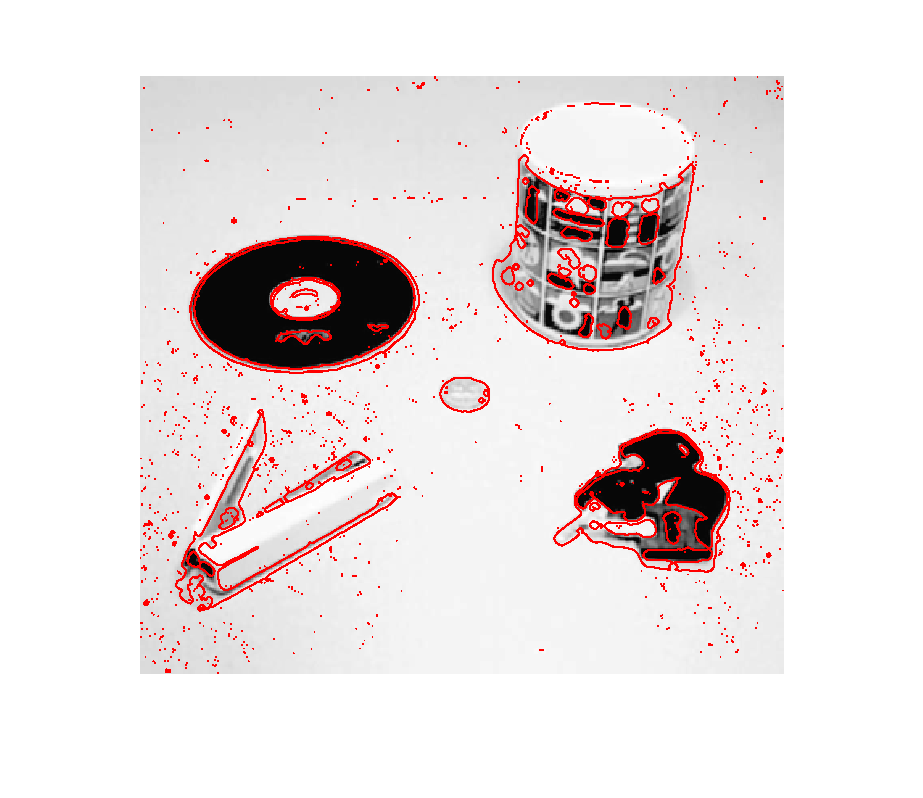
\includegraphics[width=0.45\textwidth]{../program/wenju-1.eps}}
    \subfigure[得到的边界]{
    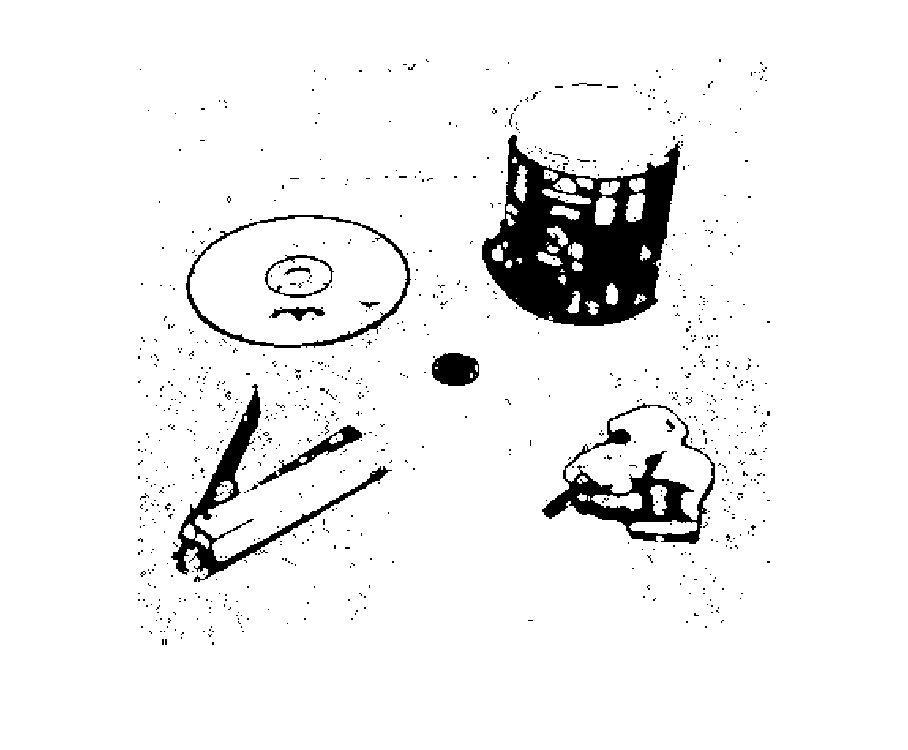
\includegraphics[width=0.45\textwidth]{../program/wenju-2.eps}}
    \subfigure[梯度图]{
    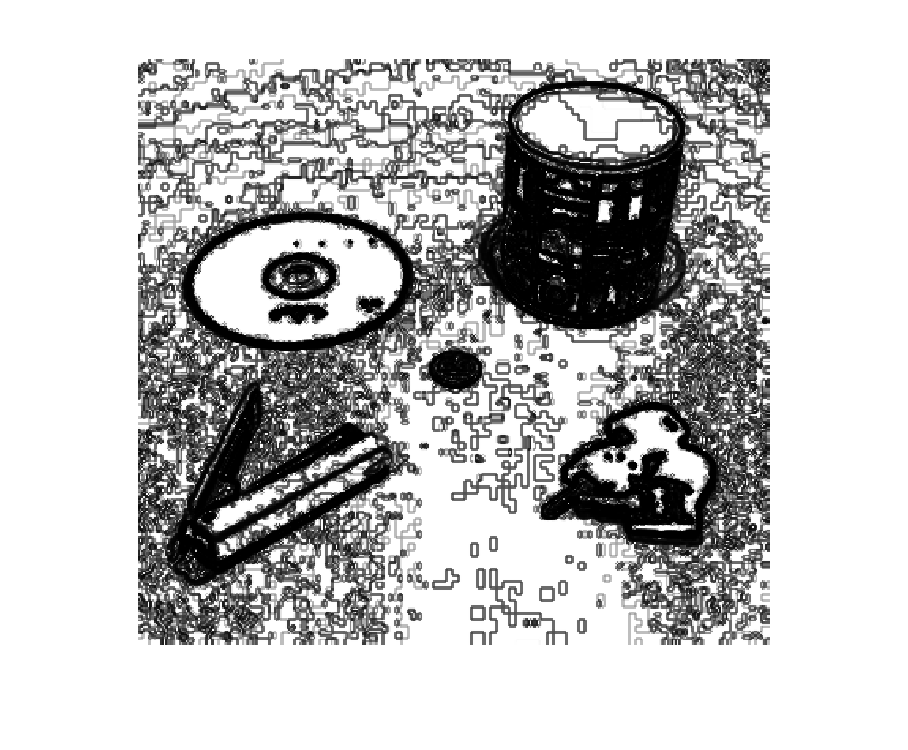
\includegraphics[width=0.45\textwidth]{../program/wenju-3.eps}}
\end{figure}
可以发现对分离图形,利用水平集方法对其进行逼近的效果较好,利用梯度也可
以大致看出图像的轮廓,但噪声较大。 \par
该例子选自课程PPT,课程PPT上的包裹曲线只在图形外部,而不会进入内部。经
过实验表明,将$dt$取得较小$dt=0.1$可以达到PPT上的效果,我个人认为包裹
曲线进入内部也未尝不可。

\subsection{人物肖像}
\begin{figure}[H]
    \centering
    \subfigure[原图]{
    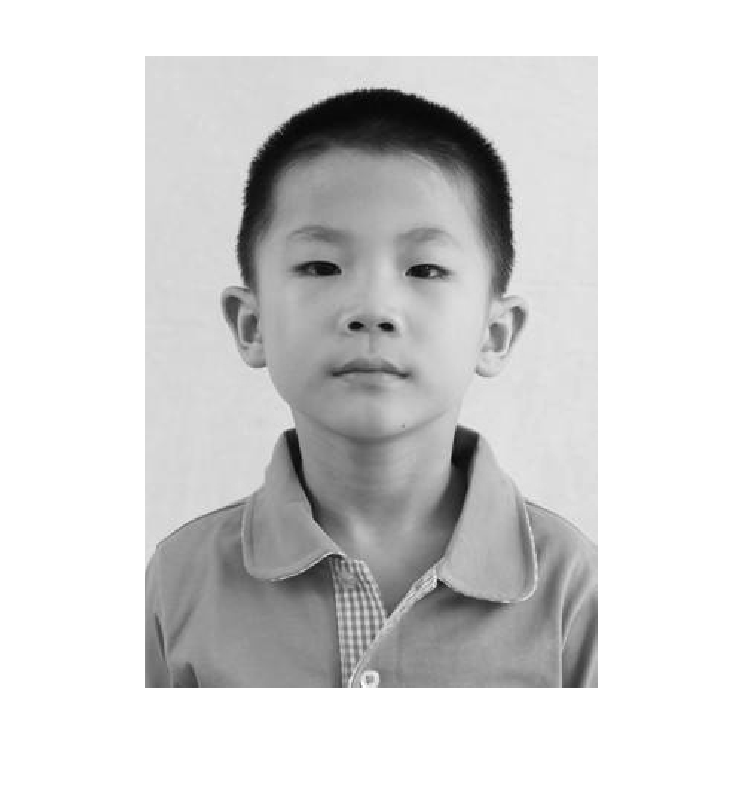
\includegraphics[width=0.45\textwidth]{../program/baby.eps}}
    \subfigure[迭代结果]{
    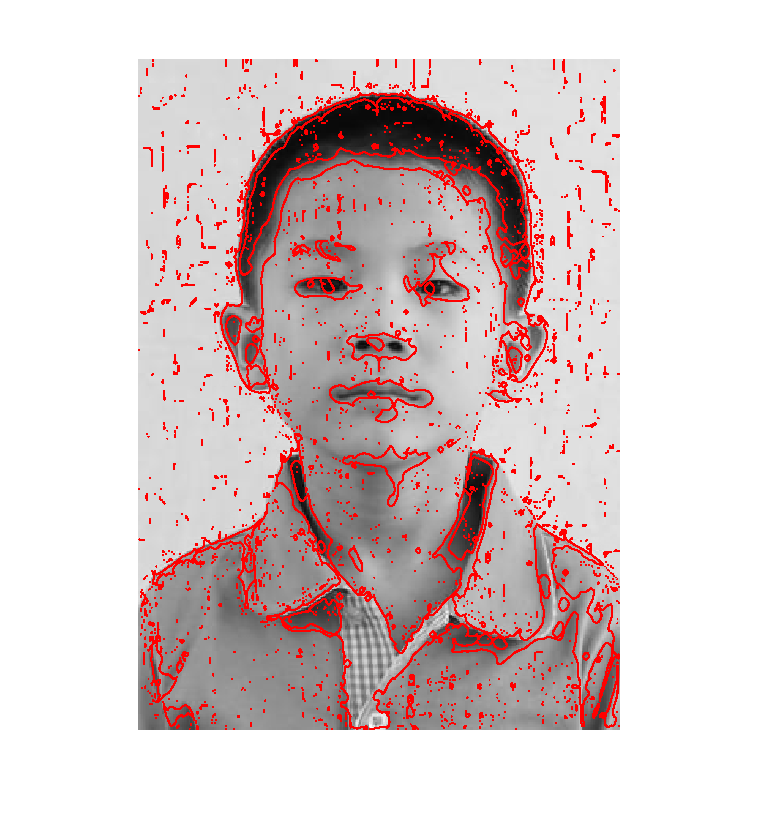
\includegraphics[width=0.45\textwidth]{../program/baby-1.eps}}
    \subfigure[得到的边界]{
    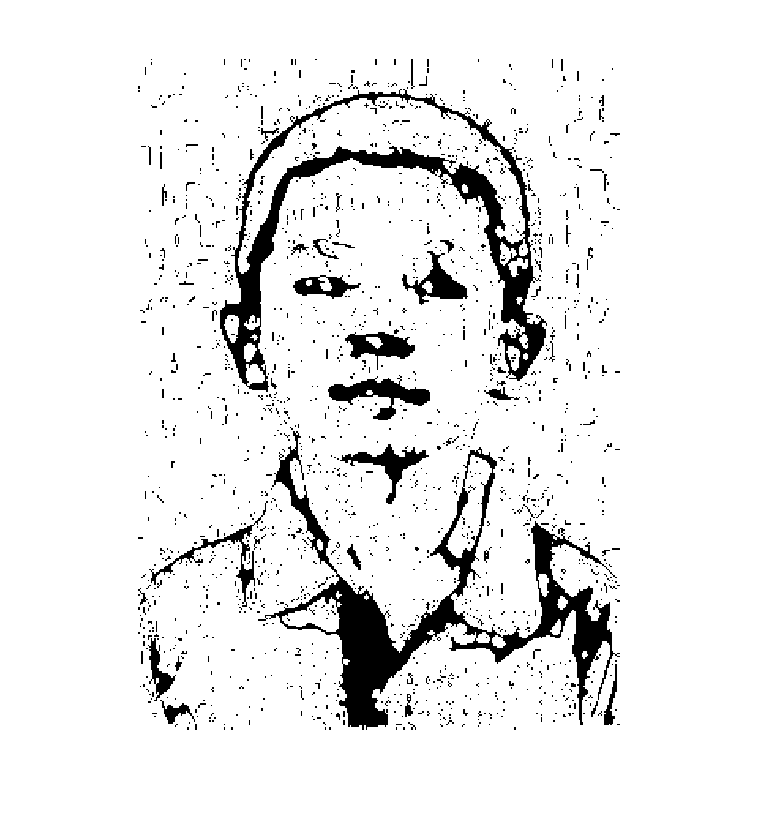
\includegraphics[width=0.45\textwidth]{../program/baby-2.eps}}
    \subfigure[梯度图]{
    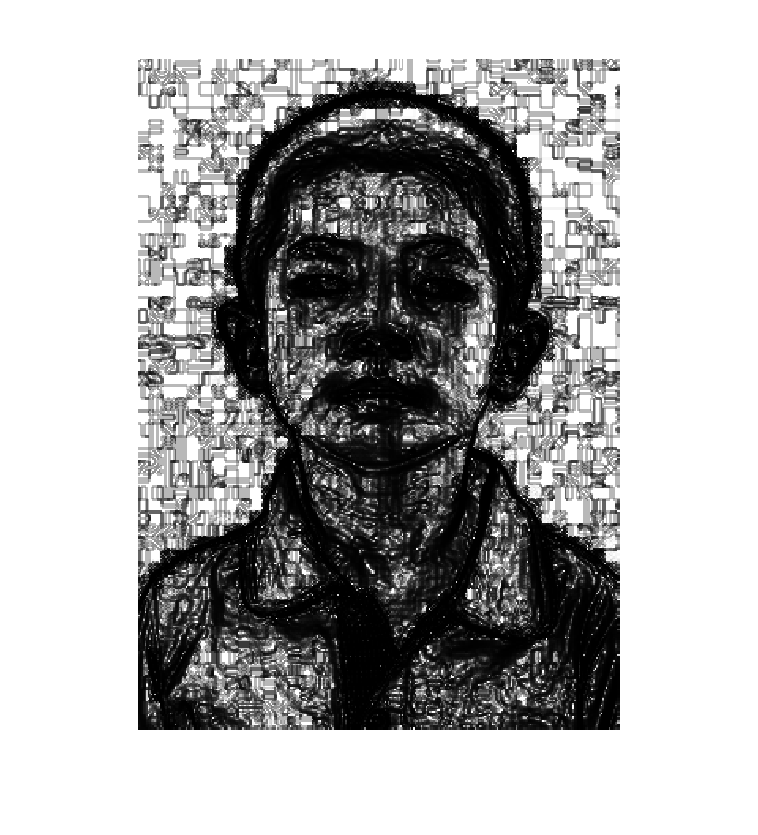
\includegraphics[width=0.45\textwidth]{../program/baby-3.eps}}
\end{figure}
可以发现对于人物肖像这种较为复杂的图形,该方法的效果会有所影响,但大致
轮廓还是能看出。而梯度图已经看不出轮廓了。
\subsection{加噪声}
我们采用以下式为卷积核的加噪声处理:
\[
k = \text{fspecial}("Gaussian",[15,15],\sigma_1).
\]
\subsubsection{少量噪声}
$\sigma_1 = 1.5$
\begin{figure}[H]
    \centering
    \subfigure[原图]{
    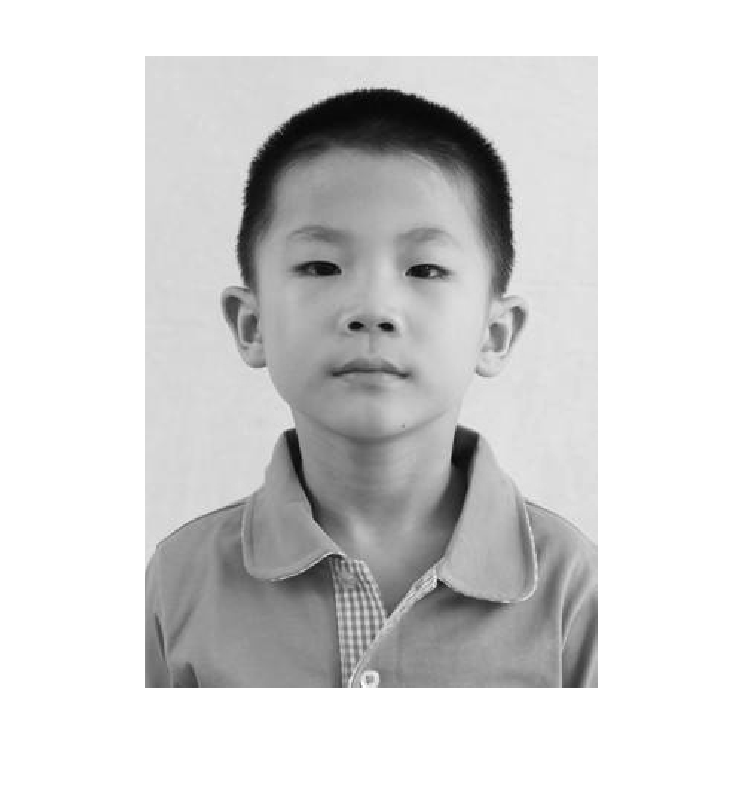
\includegraphics[width=0.45\textwidth]{../program/baby.eps}}
    \subfigure[加模糊]{
    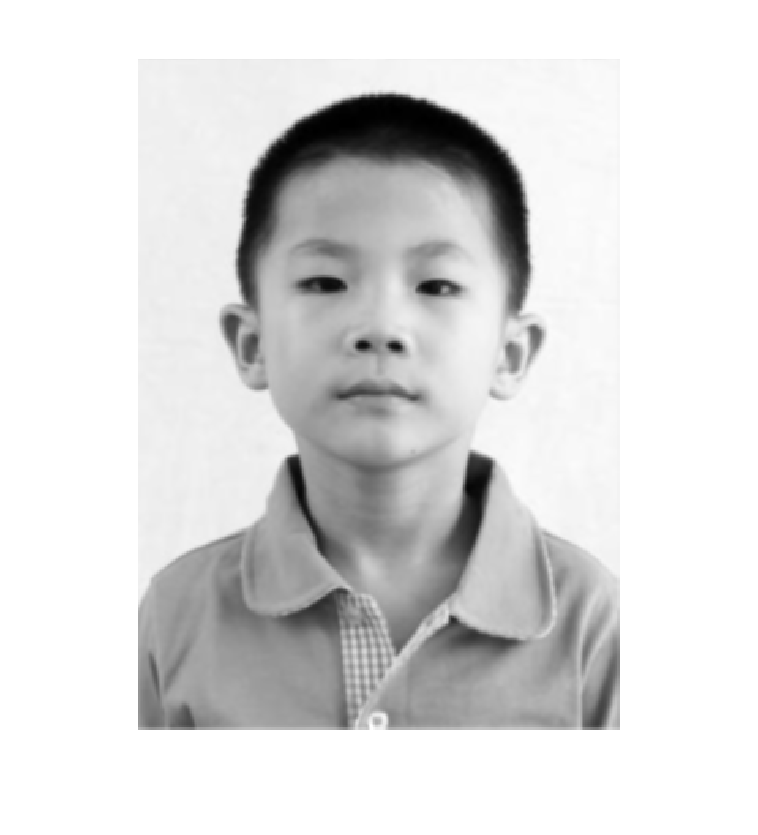
\includegraphics[width=0.45\textwidth]{../program/babyblur-1.eps}}
    \subfigure[迭代结果]{
    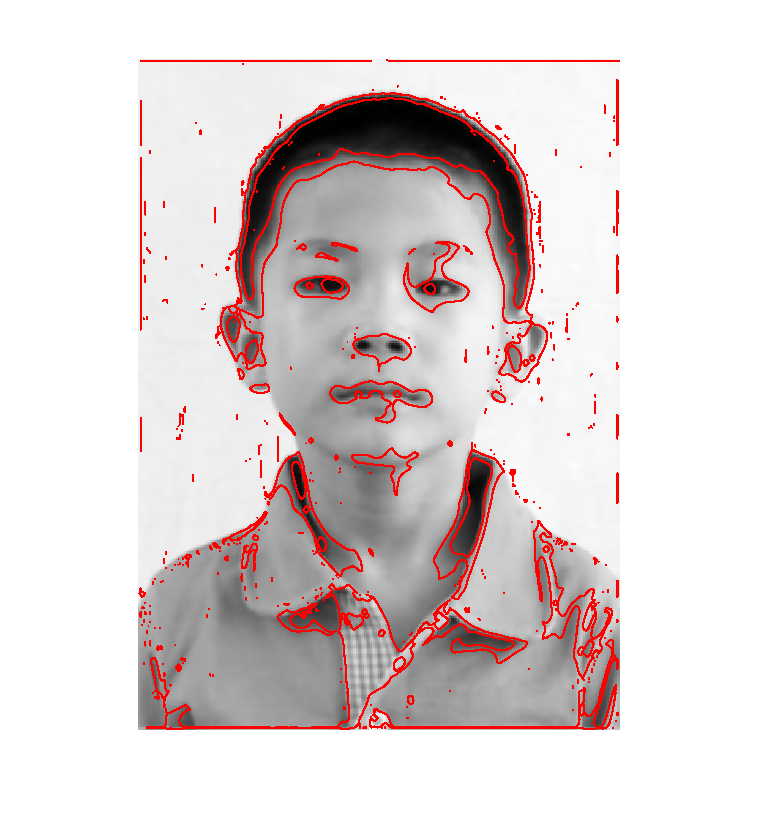
\includegraphics[width=0.45\textwidth]{../program/babyblur-2.eps}}
    \subfigure[得到的边界]{
    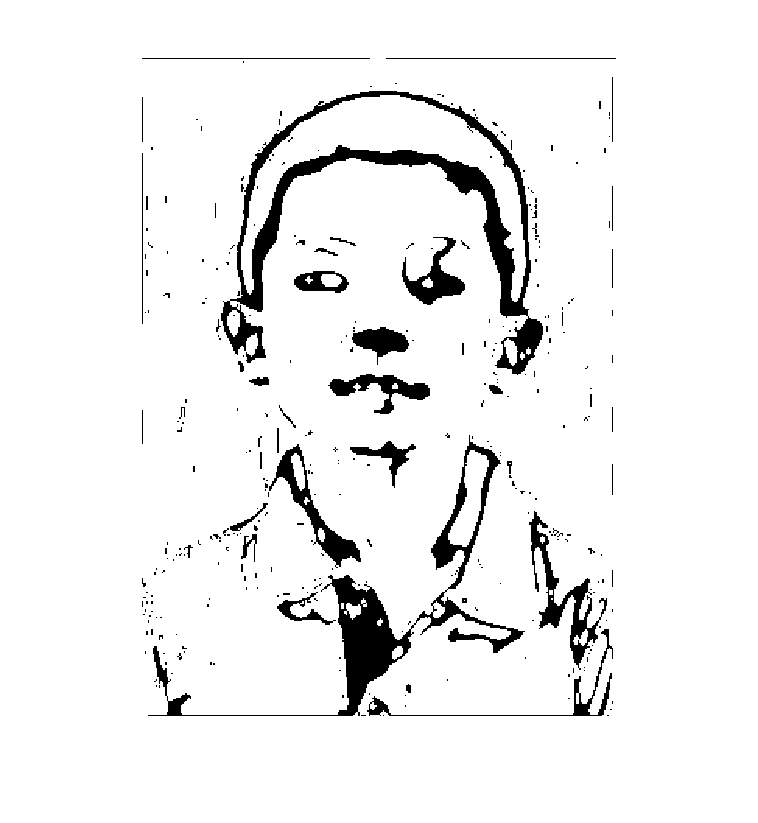
\includegraphics[width=0.45\textwidth]{../program/babyblur-3.eps}}
\end{figure}

可以发现少量噪声的存在使得捕捉到的轮廓相对于没有噪声的情形更为清晰。
\subsubsection{较多噪声}
$\sigma_1 = 5$
\begin{figure}[H]
    \centering
    \subfigure[原图]{
    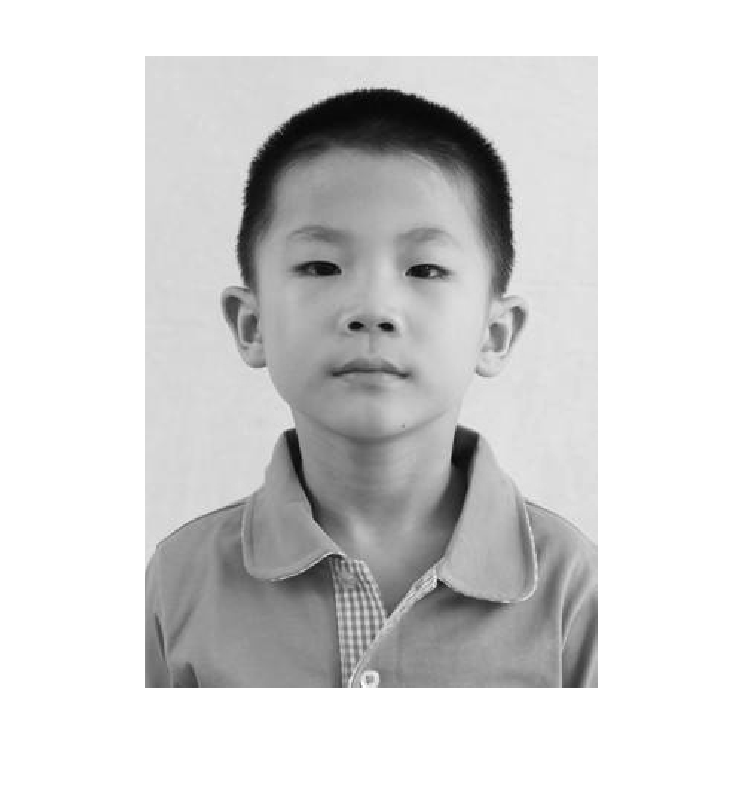
\includegraphics[width=0.45\textwidth]{../program/baby.eps}}
    \subfigure[加模糊]{
    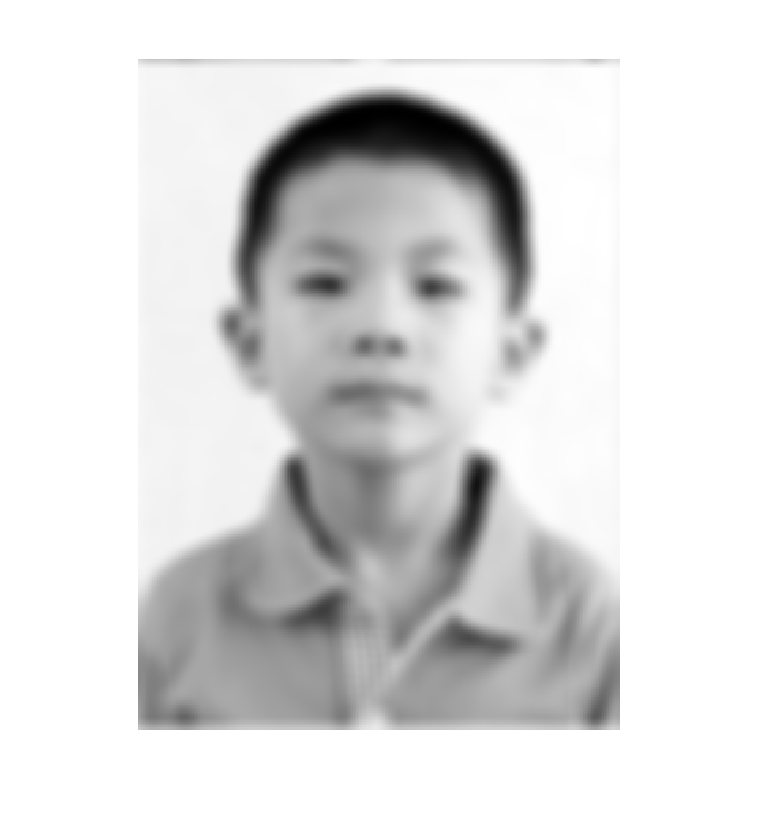
\includegraphics[width=0.45\textwidth]{../program/babyblur2-1.eps}}
    \subfigure[迭代结果]{
    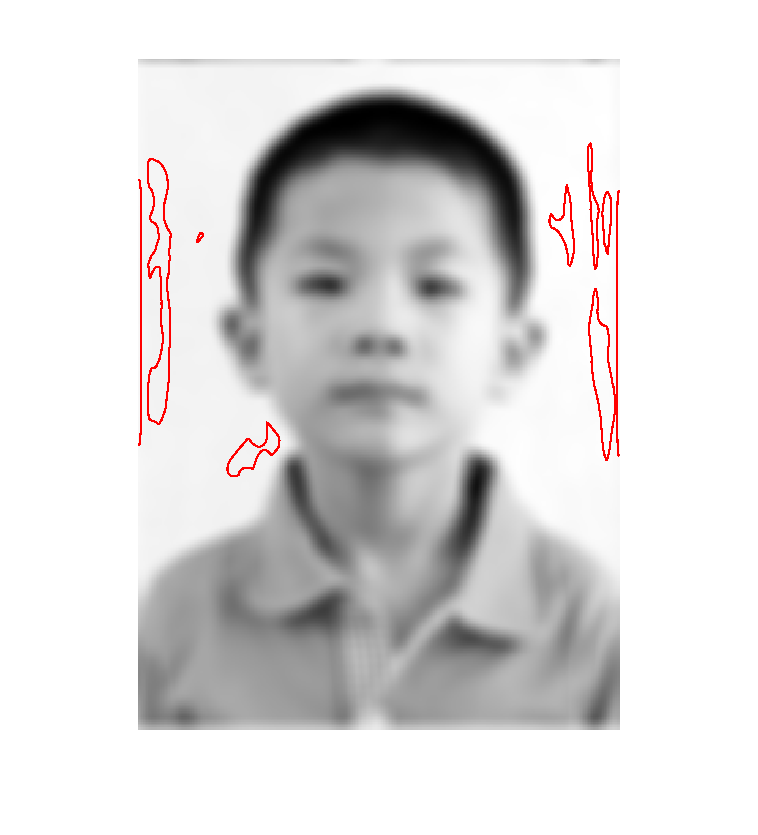
\includegraphics[width=0.45\textwidth]{../program/babyblur2-2.eps}}
    \subfigure[得到的边界]{
    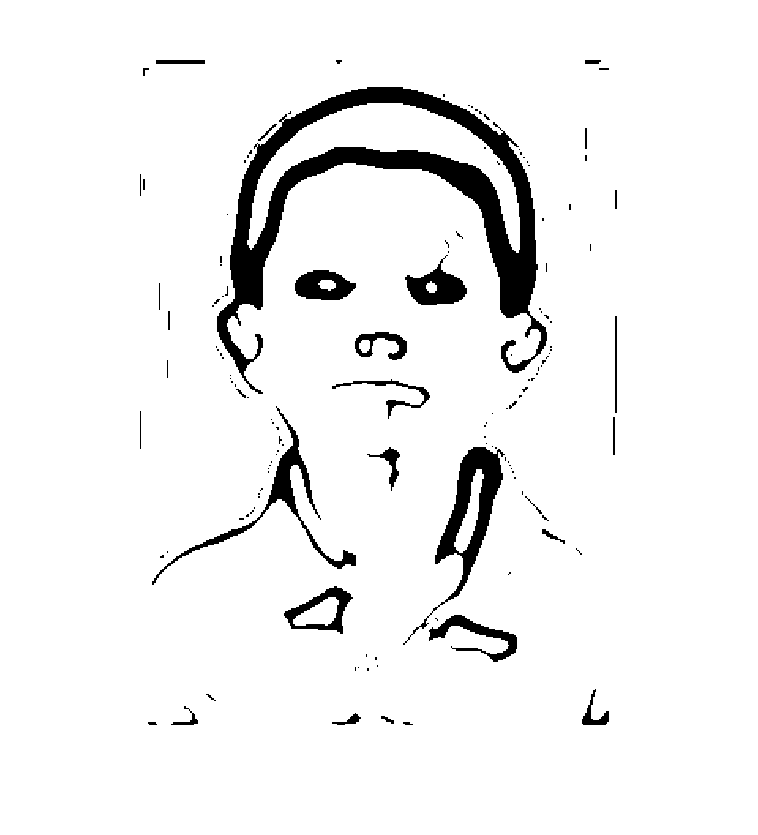
\includegraphics[width=0.45\textwidth]{../program/babyblur2-3.eps}}
\end{figure}
可以发现随着噪声增加,虽然轮廓变得更加突出,但也有部分轮廓被掩盖消失了
。

\section{上机报告总结}
本次上机报告我们采用了水平集方法实现Geodesic active contours 模型,
对图像的轮廓进行捕捉。
\par
该方法对一些简单的,分离的图形能较好的找到图形边界,但对复杂图形的效果
会打折扣。

对图形加模糊能强化图形边界,但过多的模糊会让边界无法被检出。

\end{document} 

